  \documentclass[crop,tikz]{standalone}% 'crop' is the default for v1.0, before it was 'preview'
%\usetikzlibrary{...}% tikz package already loaded by 'tikz' option
\usepackage[utf8]{inputenc}

\begin{document}
  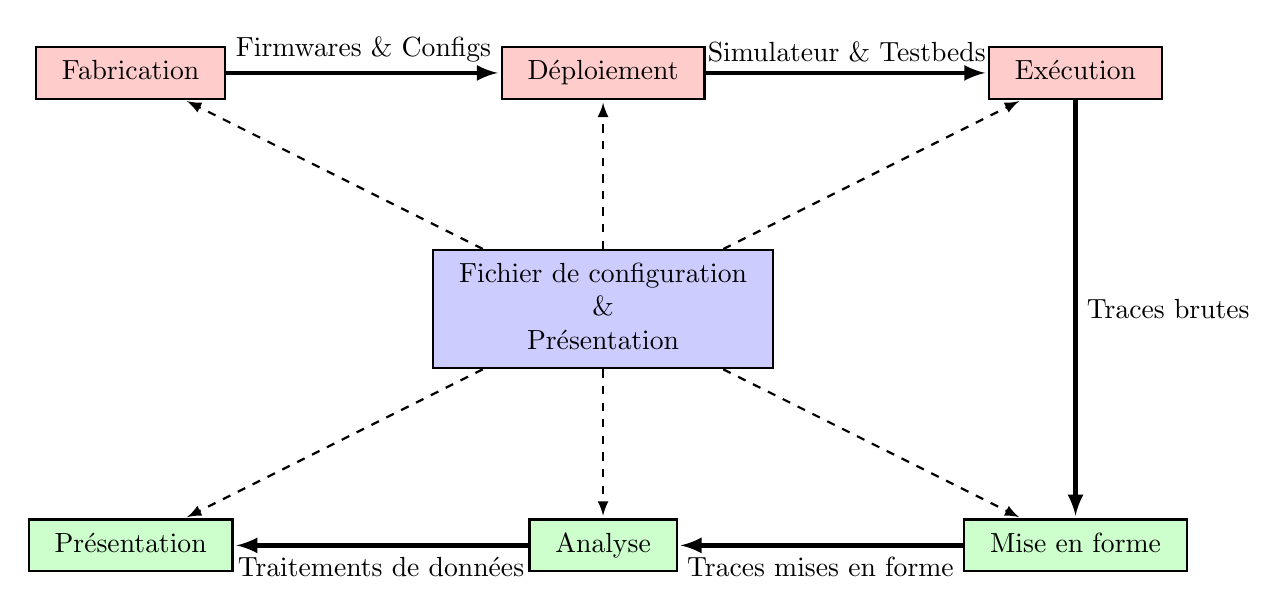
\begin{tikzpicture}[->,>=latex,shorten >=1pt,auto,node distance=3cm,
    thick,
    main node/.style={fill=blue!20,draw},
    pre node/.style={fill=red!20,draw},
    post node/.style={fill=green!20,draw}
    ]

    \node[pre node] (make) at (0, 3) {\begin{tabular}{c}Fabrication\end{tabular}};
    \node[pre node] (deploy) at (6, 3) {\begin{tabular}{c}Déploiement\end{tabular}};
    \node[pre node] (run) at (12, 3) {\begin{tabular}{c}Exécution\end{tabular}};

    \node[post node] (parse) at (12, -3) {\begin{tabular}{c}Mise en forme\end{tabular}};
    \node[post node] (analyze) at (6, -3) {\begin{tabular}{c}Analyse\end{tabular}};
    \node[post node] (plot) at (0, -3) {\begin{tabular}{c}Présentation\end{tabular}};
    
    % \node[main node] (analyze) at (12,0) {\begin{tabular}{c}Analyse\end{tabular}};

    \node[main node] (ipython) at (6,0) {\begin{tabular}{c}Fichier de configuration\\ \& \\Présentation\end{tabular}};

    \path
       (make) edge[ultra thick] node[above] {Firmwares \& Configs} (deploy) 
       (deploy) edge[ultra thick] node[above]  {Simulateur \& Testbeds} (run)
       (run) edge[ultra thick] node[right] {Traces brutes} (parse) 
       (parse) edge[ultra thick] node[below] {Traces mises en forme} (analyze)
       (analyze) edge[ultra thick] node[below] {Traitements de données} (plot)

  (ipython) edge[dashed] (make)
  (ipython) edge[dashed] (deploy)
  (ipython) edge[dashed] (run)
  (ipython) edge[dashed] (parse)
  (ipython) edge[dashed] (analyze)
  (ipython) edge[dashed] (plot)
  ;
  \end{tikzpicture}
  \end{document}